\documentclass[tikz,border=12pt]{standalone}
\usepackage[T1]{fontenc}
\usepackage{lmodern}
\usepackage{amsmath,amssymb}
\usetikzlibrary{arrows.meta,positioning}
\definecolor{ink}{HTML}{183444}
\definecolor{blue}{HTML}{1B6780}
\definecolor{amber}{HTML}{AD601A}
\definecolor{muted}{HTML}{667D88}
\begin{document}
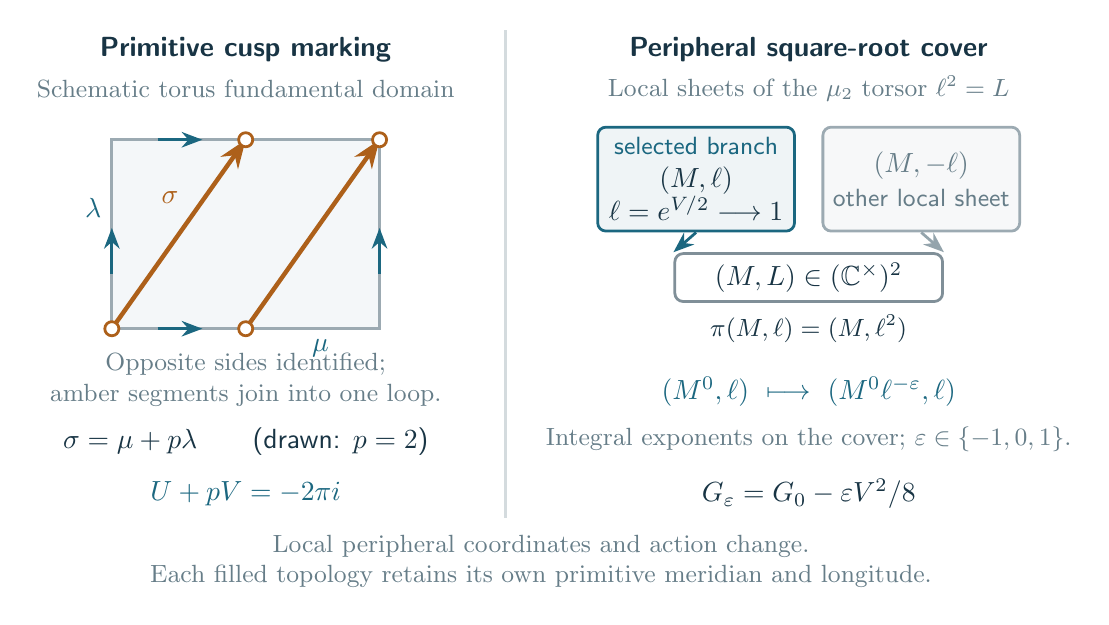
\begin{tikzpicture}[font=\sffamily,text=ink,line width=1pt,
 >=Stealth,
 point/.style={circle,draw=amber,fill=white,line width=1pt,inner sep=1.8pt},
 sheet/.style={rounded corners=3pt,draw=blue,fill=blue!7,
   minimum width=2.5cm,minimum height=.85cm,align=center},
 other/.style={sheet,draw=muted!65,fill=muted!5,text=muted}]

 % A fundamental-domain picture, deliberately not a geometric cusp shape.
 \begin{scope}[xshift=-4.15cm]
  \node at(0,3.0){\textbf{Primitive cusp marking}};
  \node[font=\small,text=muted]at(0,2.5){Schematic torus fundamental domain};
  \fill[blue!5](-1.7,-.55)rectangle(1.7,1.85);
  \draw[muted!65](-1.7,-.55)rectangle(1.7,1.85);

  % Matching arrows record the two identifications of opposite sides.
  \foreach \y in {-.55,1.85}{
   \draw[blue,->](-1.12,\y)--(-.55,\y);
  }
  \foreach \x in {-1.7,1.7}{
   \draw[blue,->](\x,.15)--(\x,.73);
  }
  \node[blue,below]at(.95,-.55){$\mu$};
  \node[blue,left]at(-1.7,.99){$\lambda$};

  % The primitive class (1,2) closes after the top/bottom identification.
  \draw[amber,line width=1.6pt,->](-1.7,-.55)--(0,1.85);
  \draw[amber,line width=1.6pt,->](0,-.55)--(1.7,1.85);
  \foreach \p in {(-1.7,-.55),(0,1.85),(0,-.55),(1.7,1.85)}{
   \node[point]at\p{};
  }
  \node[amber,above left]at(-.72,.9){$\sigma$};
  \node[font=\small,text=muted,align=center]at(0,-1.2)
    {Opposite sides identified;\\amber segments join into one loop.};
  \node at(0,-1.98){$\sigma=\mu+p\lambda\qquad\text{(drawn: }p=2\text{)}$};
  \node[blue]at(0,-2.65){$U+pV=-2\pi i$};
 \end{scope}

 \draw[muted!28](-.85,-2.95)--(-.85,3.25);

 % A LOCAL picture: the double cover is not globally split into two sheets.
 \begin{scope}[xshift=3.0cm]
  \node at(0,3.0){\textbf{Peripheral square-root cover}};
  \node[font=\small,text=muted]at(0,2.5)
    {Local sheets of the $\mu_2$ torsor $\ell^2=L$};
  \node[sheet,minimum height=1.32cm](selected)at(-1.43,1.35)
    {\textcolor{blue}{\small selected branch}\\$(M,\ell)$\\$\ell=e^{V/2}\longrightarrow 1$};
  \node[other,minimum height=1.32cm](other)at(1.43,1.35)
    {$(M,-\ell)$\\{\small other local sheet}};
  \node[draw=ink!55,rounded corners=3pt,fill=white,
        minimum width=3.4cm,minimum height=.55cm](base)at(0,.1)
    {$(M,L)\in(\mathbb C^\times)^2$};
  \draw[blue,->](selected.south)--(base.north west);
  \draw[muted!70,->](other.south)--(base.north east);
  \node[font=\small]at(0,-.55)
    {$\pi(M,\ell)=(M,\ell^2)$};
  \node[blue]at(0,-1.35)
    {$(M^0,\ell)\ \longmapsto\ (M^0\ell^{-\varepsilon},\ell)$};
  \node[font=\small,text=muted]at(0,-1.95)
    {Integral exponents on the cover; $\varepsilon\in\{-1,0,1\}$.};
  \node at(0,-2.65){$G_{\varepsilon}=G_0-\varepsilon V^2/8$};
 \end{scope}

 \node[font=\small,text=muted,align=center]at(-.4,-3.5)
   {Local peripheral coordinates and action change.\\
    Each filled topology retains its own primitive meridian and longitude.};
\end{tikzpicture}
\end{document}
